\documentclass[10pt,twocolumn]{article}

% use the oxycomps style file
\usepackage{oxycomps}
\usepackage[table]{xcolor}

% usage: \fixme[comments describing issue]{text to be fixed}
% define \fixme as not doing anything special
\newcommand{\fixme}[2][]{#2}
% overwrite it so it shows up as red
\renewcommand{\fixme}[2][]{\textcolor{red}{#2}}
% overwrite it again so related text shows as footnotes
%\renewcommand{\fixme}[2][]{\textcolor{red}{#2\footnote{#1}}}

% read references.bib for the bibtex data
\bibliography{references}

% include metadata in the generated pdf file
\pdfinfo{
    /Title (Scanning Books Utilizing Stationary Videos: Project Proposal)
    /Author (John J. Kim)
}

% set the title and author information
\title{Scanning Books Utilizing Stationary Videos: Project Proposal}
\author{John J. Kim}
\affiliation{Occidental College}

\email{jkim4@oxy.edu}
 
\begin{document}

\maketitle

\section{Introduction}

Scanning documents from images allows users to easily digitize physical mediums without  using more tedious, time-consuming, and costly photo-scanners\cite{luqman2014}. It also allows users to minimize contact with the medium, making it ideal for the purposes of archival. Today, in the ongoing struggles of mass digitization of archival documents, a tool that allows archivists to easily and reliably digitize the material is crucial in the interest of archival preservation. Though there are several images to pdf scanners commercially available today, no video to pdf scanner is available \cite{lesure2016}. This paper aims to develop a software that allows documents to be scanned from a video, streamlining this process, allowing users to easily and quickly scan hundreds if not thousands of pages continuously. \newline

\section{Technical Background}

Today, in the ongoing struggles of mass digitization of archival documents\cite{miller2013}, a tool that allows archivists to easily and reliably digitize the material is crucial in the interest of archival preservation.\newline

The lack of digitization of pre-digital age texts and documents have long hindered historical research, as often a source cannot be confirmed if it is not digitally available, forcing researchers to purchase the material at an absurd price point, if it's even available for purchase, visit a major library with an inconceivably large collection, or–and more often than not–blindly trust the citation\cite{blessing2023}.\newline

I aim to develop a program that allows users to scan physical mediums with a stationary video of it utilizing cloud computing. The ease of use of the program will aid in addressing the enormous backlog of archival text yet to be digitized\cite{kleber2017}, while preserving the quality of the digital scans as much as possible. The program will never be able to replace or out-perform traditional scanning methods, but it’ll be the most non-envasive method of scanning and will deliver comparable quality, ease of use, and at no cost, allowing smaller libraries and individual owners to digitize mediums.\newline

\subsection{Scanning Books from Images/Videos}

Scanning a book from images/videos can be much more difficult than scanning documents or pamphlets. A two dimensional paper on a flat surface can be scanned by only identifying the four edges, but a book needs to identify the curve caused by the book spine and morph the image accordingly\cite{jiang2015}. Also, sections of the page could also be hidden by the spin curve, making it impossible to scan the whole page\cite{wigington2024}.\newline


\subsection{Adobe Scan App}

These so-called "scan apps" are experiencing mass adoption due to their shear convenience compared to using a clunky scanner\cite{permana2020}. Adobe Scan is one of the best commercially available "scan app" in regards to book scanning with a phone\cite{keough2024}. Their book scan feature is only available with the premium plan. It can handle the spine curve quite well and can scan both pages simultaneously, but it can only accept images; Also, it only scans individual pages as individual pages leading to inconsistent margins.\newline

\subsection{Adobe Paper}

Adobe recently published a paper attempting to scan books with a video feed utilizing the PUCIT dataset\cite{wigington2024}. Unfortunately, their software is not currently commercially available as the results show that it performed inconsistently.\newline

The Adobe paper primarily limited by two factors that do not affect my project: they utilize local computing on the phone, presumably due to the high server maintenance costs that would entail considering their large user base, and non-stationary camera feed for ease of use for the average user. The user base won't be large enough to overload the server as the program will be primarily for archival use. Also, the non-stationary camera feed requires additional computational power. Since my user base will be primarily those in the field of academia, it is not unreasonable for the program to mandate a tripod. \newline

Furthermore, the paper limit the feed between 20-40 FPS, depending on the processing power of the phone, in order to maintain real-time processing, which is undoubtedly at the cost of the scan quality. It is absurd to limit FPS when identifying the best images and scanning it is so crucial to the quality of the scan but is understandable as the average user wouldn’t want to use their phone as a server for any length of time. Adobe is developing this new feature to be local and real-time at the great cost of the scan quality. In fact, the Adobe paper fails to present a single example of a scanned document through the video format. My program, since the primary purpose is archival, will aim to preserve scan quality as much as possible.\newline


\section{Implementation}

My primary concern is with the implementation of “page change” and “hand over content”\cite{wigington2024}. I could do this in several ways.\newline

I could identify the best images of every half-second and scan it regardless of page change and stitch the pages together using the page number or identifying the duplicates using the text it-self, assuming it has a page number. Such a brute force method will be horribly inefficient, but computational power is not a limiting factor. My upper-limit goal is to achieve 0.5-minute per page, meaning a 300 page book will take about 2.5 hrs.\newline

I could have the user flash a qr code to indicate completion of page change. This method hinders ease of use and makes the program susceptible to human error. But admittedly, this will be, by far, the easiest to implement.\newline

I could do what Adobe did and conduct machine learning to identify page change event, utilizing the PUCIT Page Turn dataset.\newline

I could also implement hand detection and assume a page change is completed when a hand is no longer visible in the video feed. The reliability of the hand detection must be highly accurate and consistent to prevent a page skin event. The hand detection algorithm must be trained on a racially diverse dataset to ensure that people of all skin tones can use the program. Furthermore, gloves are often used in handling fragile documents and the program must be able to detect gloves of all types and colors.\newline

Regardless of the method I will double check the page numbers to ensure no page turn was missed.\newline

Developing machine learning to locate the spine is unnecessary, as since the video is stationary we can ask the user to locate the line that separates the two pages.\newline

\subsection{Optical Character Recognition (OCR)}

The scanner apps are often capable of Optical Character Recognition(OCR) to make the document machine readable and editable. Due to inconsistencies in formatting, fonts, and image quality, modern OCR utilizes deep learning in development\cite{hukkeri2022}. Developing a reliable OCR through deep learning requires an “enormous amount of data”\cite{hukkeri2022}.\newline

Google Cloud Vision(GCV) and Intel's OpenCV are one of dominant players in real-time computer vision. OpenCV, unlike GCV, is free under the Apache License. And the Library for OpenCV can easily be imported in python to process the video and can be used with another library in conjunction called Tesseract(an open-source OCR engine).\newline

OCR can aid in scanning through images and videos as it allows identification where the texts are, relative to the camera, aiding in evaluating the margins\cite{avyodri2022}. It’ll especially be useful for page number detection. It's also good quality of life feature in general.\newline

\subsection{OpenCV}
In python's vast ecosystem there are countless packages serve various functions. OpenCV (Open Source Computer Vision Library) is one such program that is written in multiple languages, including Python. It is a very well established real time computer vision program developed and managed by intel. Although it is not designed for scanning documents, it is very useful for managing/processing videos. In the context of this paper, it'll be used to detect the “page change” and “hand over content” events\cite{wigington2024}, utilizing motion detection and hand detection, then capturing/cropping images of the book based on the events and the given location of the book spine.\newline

OpenCV is also under the Apache License, which essentially means it's in the public domain prematurely and voluntarily. Hence, I can use it for my project without worrying about licensing or royalties.\newline

\subsection{Tesseract}
Tesseract is a highy reliable and reputable open source Optical Character Recognition(OCR) program with a long history. It was initially developed as a proprietary software in the 1980's, released in 2005 as an open source project, and is supported to this day. In fact Google was involved in its development in 2006 soon after the project became open source\cite{vincent2006}. Though it is written in C++, the library can easily be imported in python and used with OpenCV. It currently supports recognition of 66 languages, including a few right-to-left languages such as Arabic and Hebrew. Also, the program is under the Apache License.\newline

\begin{figure}
    \centering
    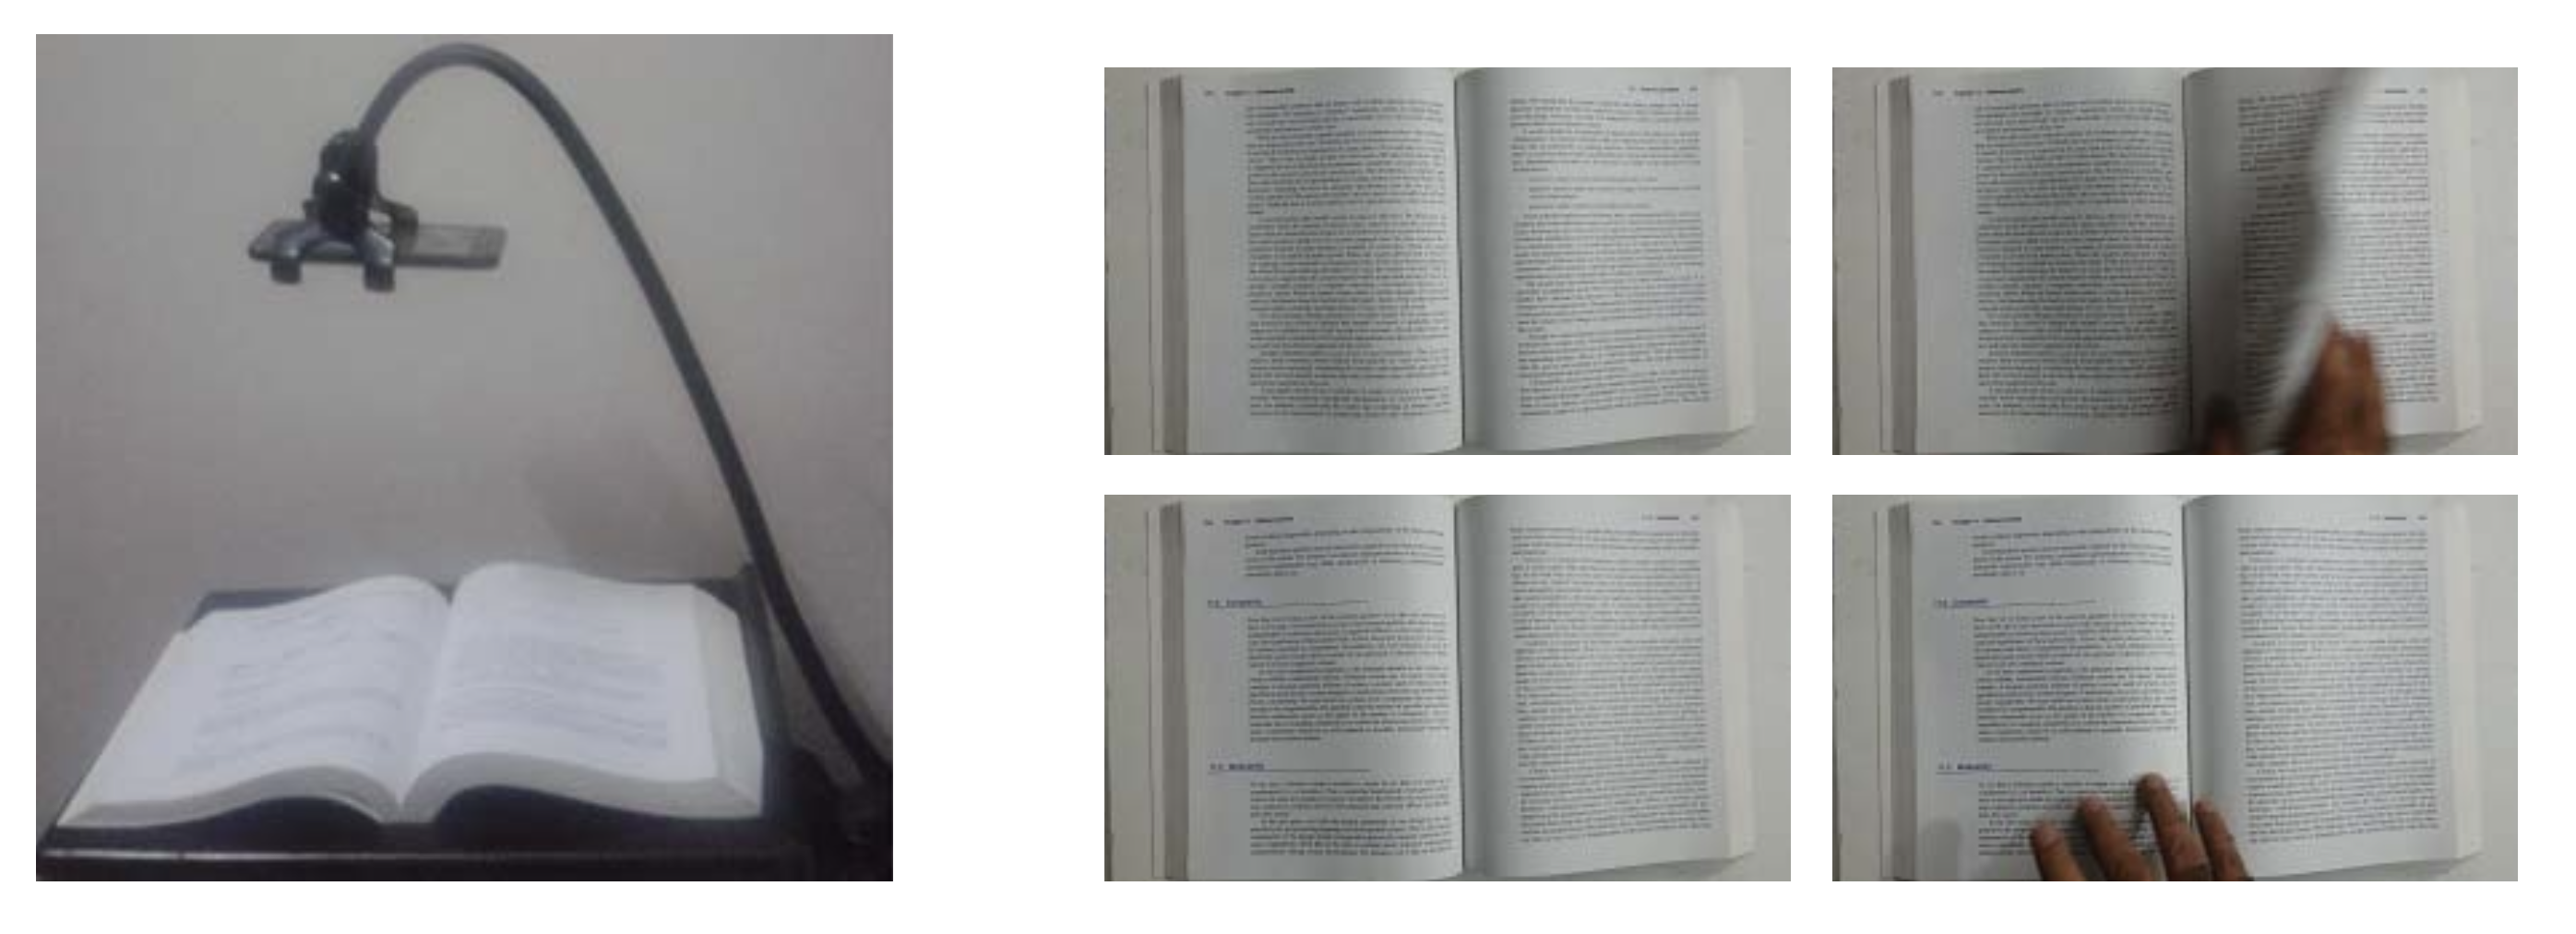
\includegraphics[width=1\linewidth]{PUCIT.png}
    \caption{PUCIT Dataset Setup}
    \label{fig:enter-label}
\end{figure}

\subsection{P.U.C.I.T. dataset}
The PUCIT(Punjab University College of Information Technology) dataset consists of top down footage of a person flipping through a book and documents. To elaborate, the dataset consists of 37 videos, 35 books and 2 documents, consisting of manually annotated 763 Page Turn Events(PTTEs)\cite{tariq2017}.\newline

It was published with a 2017 paper calling for the development of "a click-free method for video-based digitization of multi-page documents" \cite{tariq2017}. It is "only publicly available dataset for document video capture"\cite{wigington2024}. It was recorded with a Samsung Galaxy Grand Prime with a resolution of 1920×1080 pixels, but was scaled down to 480×270 pixels "for faster processing". The footage is recorded without any additional illuminations as to simulate an accurate use case conditions.\newline

\subsection{DocUNet}
A number of professors at Stony Brooks University were able to develop a "Document Image Unwrapping" program by training a DocUNet(Document U-shaped Network) neural network under the MIT License utilizing images of crumpled documents and images of their backgrounds\cite{ma2018}\cite{zhang2021}. Their model was able to "unwrap" paper folds and creases of documents.\newline 

I am curious how their model will perform trained on an image of the book and of the background, but unfortunately I currently lack the processing power to train and test the model. [Note to Professor: this won't be a problem in the fall. I'll bring my desktop from home.] I believe the model can be trained to perform effectively on books with the PUCIT page turn dataset\cite{wigington2024}.  Admittedly this is not exactly a large data set and will require a photo-shopped image of the background. Also the data set is on modern books which is not representative of yet to be digitized books of archival value. Since Adobe developed their aforementioned program utilizing this dataset and considering the limited size of the dataset, it is not inconceivable for me to develop my own dataset comparable to the PUCIT dataset.\newline

In conclusion, I plan to train the Stony Brooks model of DocUNet, utilizing the PUCIT page turn dataset and my own, if that proves to be necessary. I believe such a model will be able to scan images of books on white-monochrome background (the background used in PUCIT dataset).\newline

\subsection{page-dewarp}
\texttt{page-dewarp} is a modification of \texttt{page\_dewarp}, which was originally published by Matt Zucker in 2016 through a blog post\cite{}. \texttt{page-dewarp}, is still supported and is compatible with python3, unlike \texttt{page\_dewarp}. In fact, \texttt{page-dewarp} can even be installed as a pip.\newline

The code(s) are/is under the MIT License, which is a more informal version of the Apache License. It is "[a] short and simple permissive license with conditions only requiring preservation of copyright and license notices." \texttt{page-dewarp} honored the MIT License by preserving the plain text file containing the license, fulfilling their one and only obligation to the initial author.\newline

\texttt{page-dewarp}, like \texttt{page\_dewarp}, aims to dewarp the spine curve of images of books. However, the code is unwieldily. It often fails to detect a page and refuses to output a scan or the scan is over-warped. It cannot scan pages with large images, diagrams, or charts. In fact, both \texttt{page-dewarp} and \texttt{page\_dewarp} fails to scan one of the sample test image that contains a large spread sheet rotated 90 degrees that covers the whole page. \newline

If I can modify the code to be more consistent with its scans, it could present an interesting avenue in developing my project. \newline

\subsection{img2pdf}
img2pdf is a simple file conversion python package that can convert various different types of image files to a pdf file in a lossless manner. Among its features is the combine feature which allows users combine series of image files into a single pdf file. Since my code outputs large volumes of image files to an empty folder the combine feature is useful for the project. Also \texttt{page-dewarp} outputs as a png file so the file conversion to pdf is also useful for the project.\newline

\begin{figure}
    \centering
    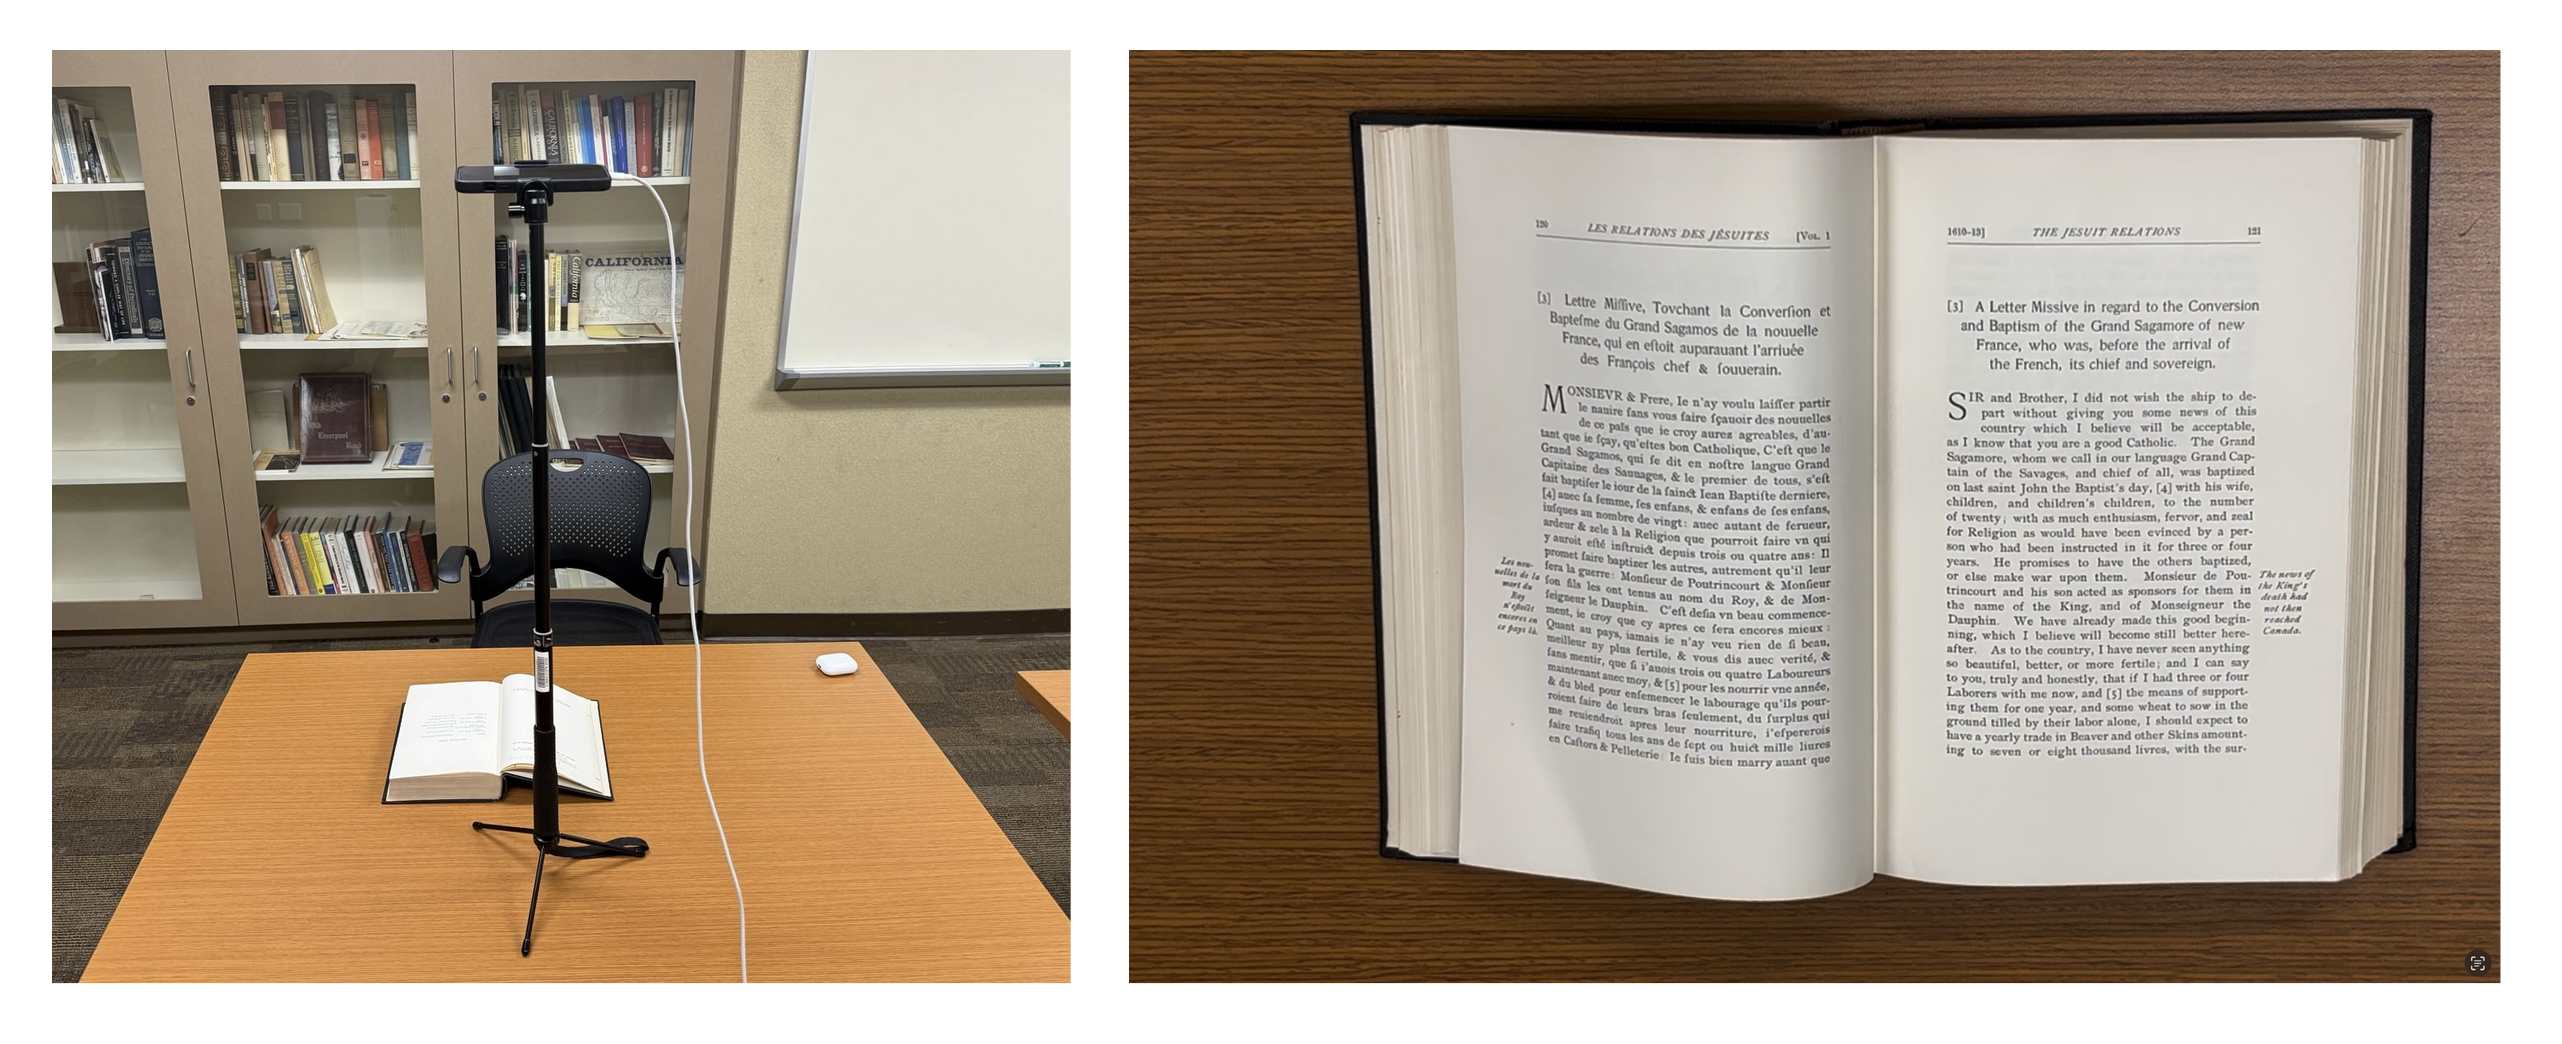
\includegraphics[width=1\linewidth]{mySetup.png}
    \caption{Proof of Concept Setup}
    \label{fig:enter-label}
\end{figure}


\section{Proof of Concept}
\noindent{\url{https://github.com/PurpleL0tus/JohnKimComps}}\newline

For the proof of concept, first I recorded a top down footage of \title{The Jesuit Relations and Allied Documents: Travels and Exploration of the Jesuit Missionaries in New France 1610-1971 Vol I} edited by Reuben G. Thwaites and published 1896. It is a approximately 660 page hard bound book with images and diagrams. I recorded the video in a manner that the PTE occured every 8 seconds exactly (I had a beeper on loop). It was a 45 minute video of me flipping through the pages in a similar fashion to the PUCIT dataset. Utilizing OpenCV, I was able to capture and crop 2 images per capture(left and right pages), though pages 262 - 352 had varying degrees of my hand in the picture due to human error.\newline

Then I ran the images through \texttt{page-dewarp}, a python package specifically designed to convert images of books to pdf by dewarping the spin curve. Only 171 of about 600 scannable pages were scanned and even scanned pages were sub-optimal. Approximately half of them had grossly over-warped leading to diagonal margins. Also all pages including pictures and diagrams failed to scan. I ran the program again which resulted in an identical scan of 171 pages consisting of exactly 3,491,703 bytes. The program is consistent.\newline

\begin{figure}
    \centering
    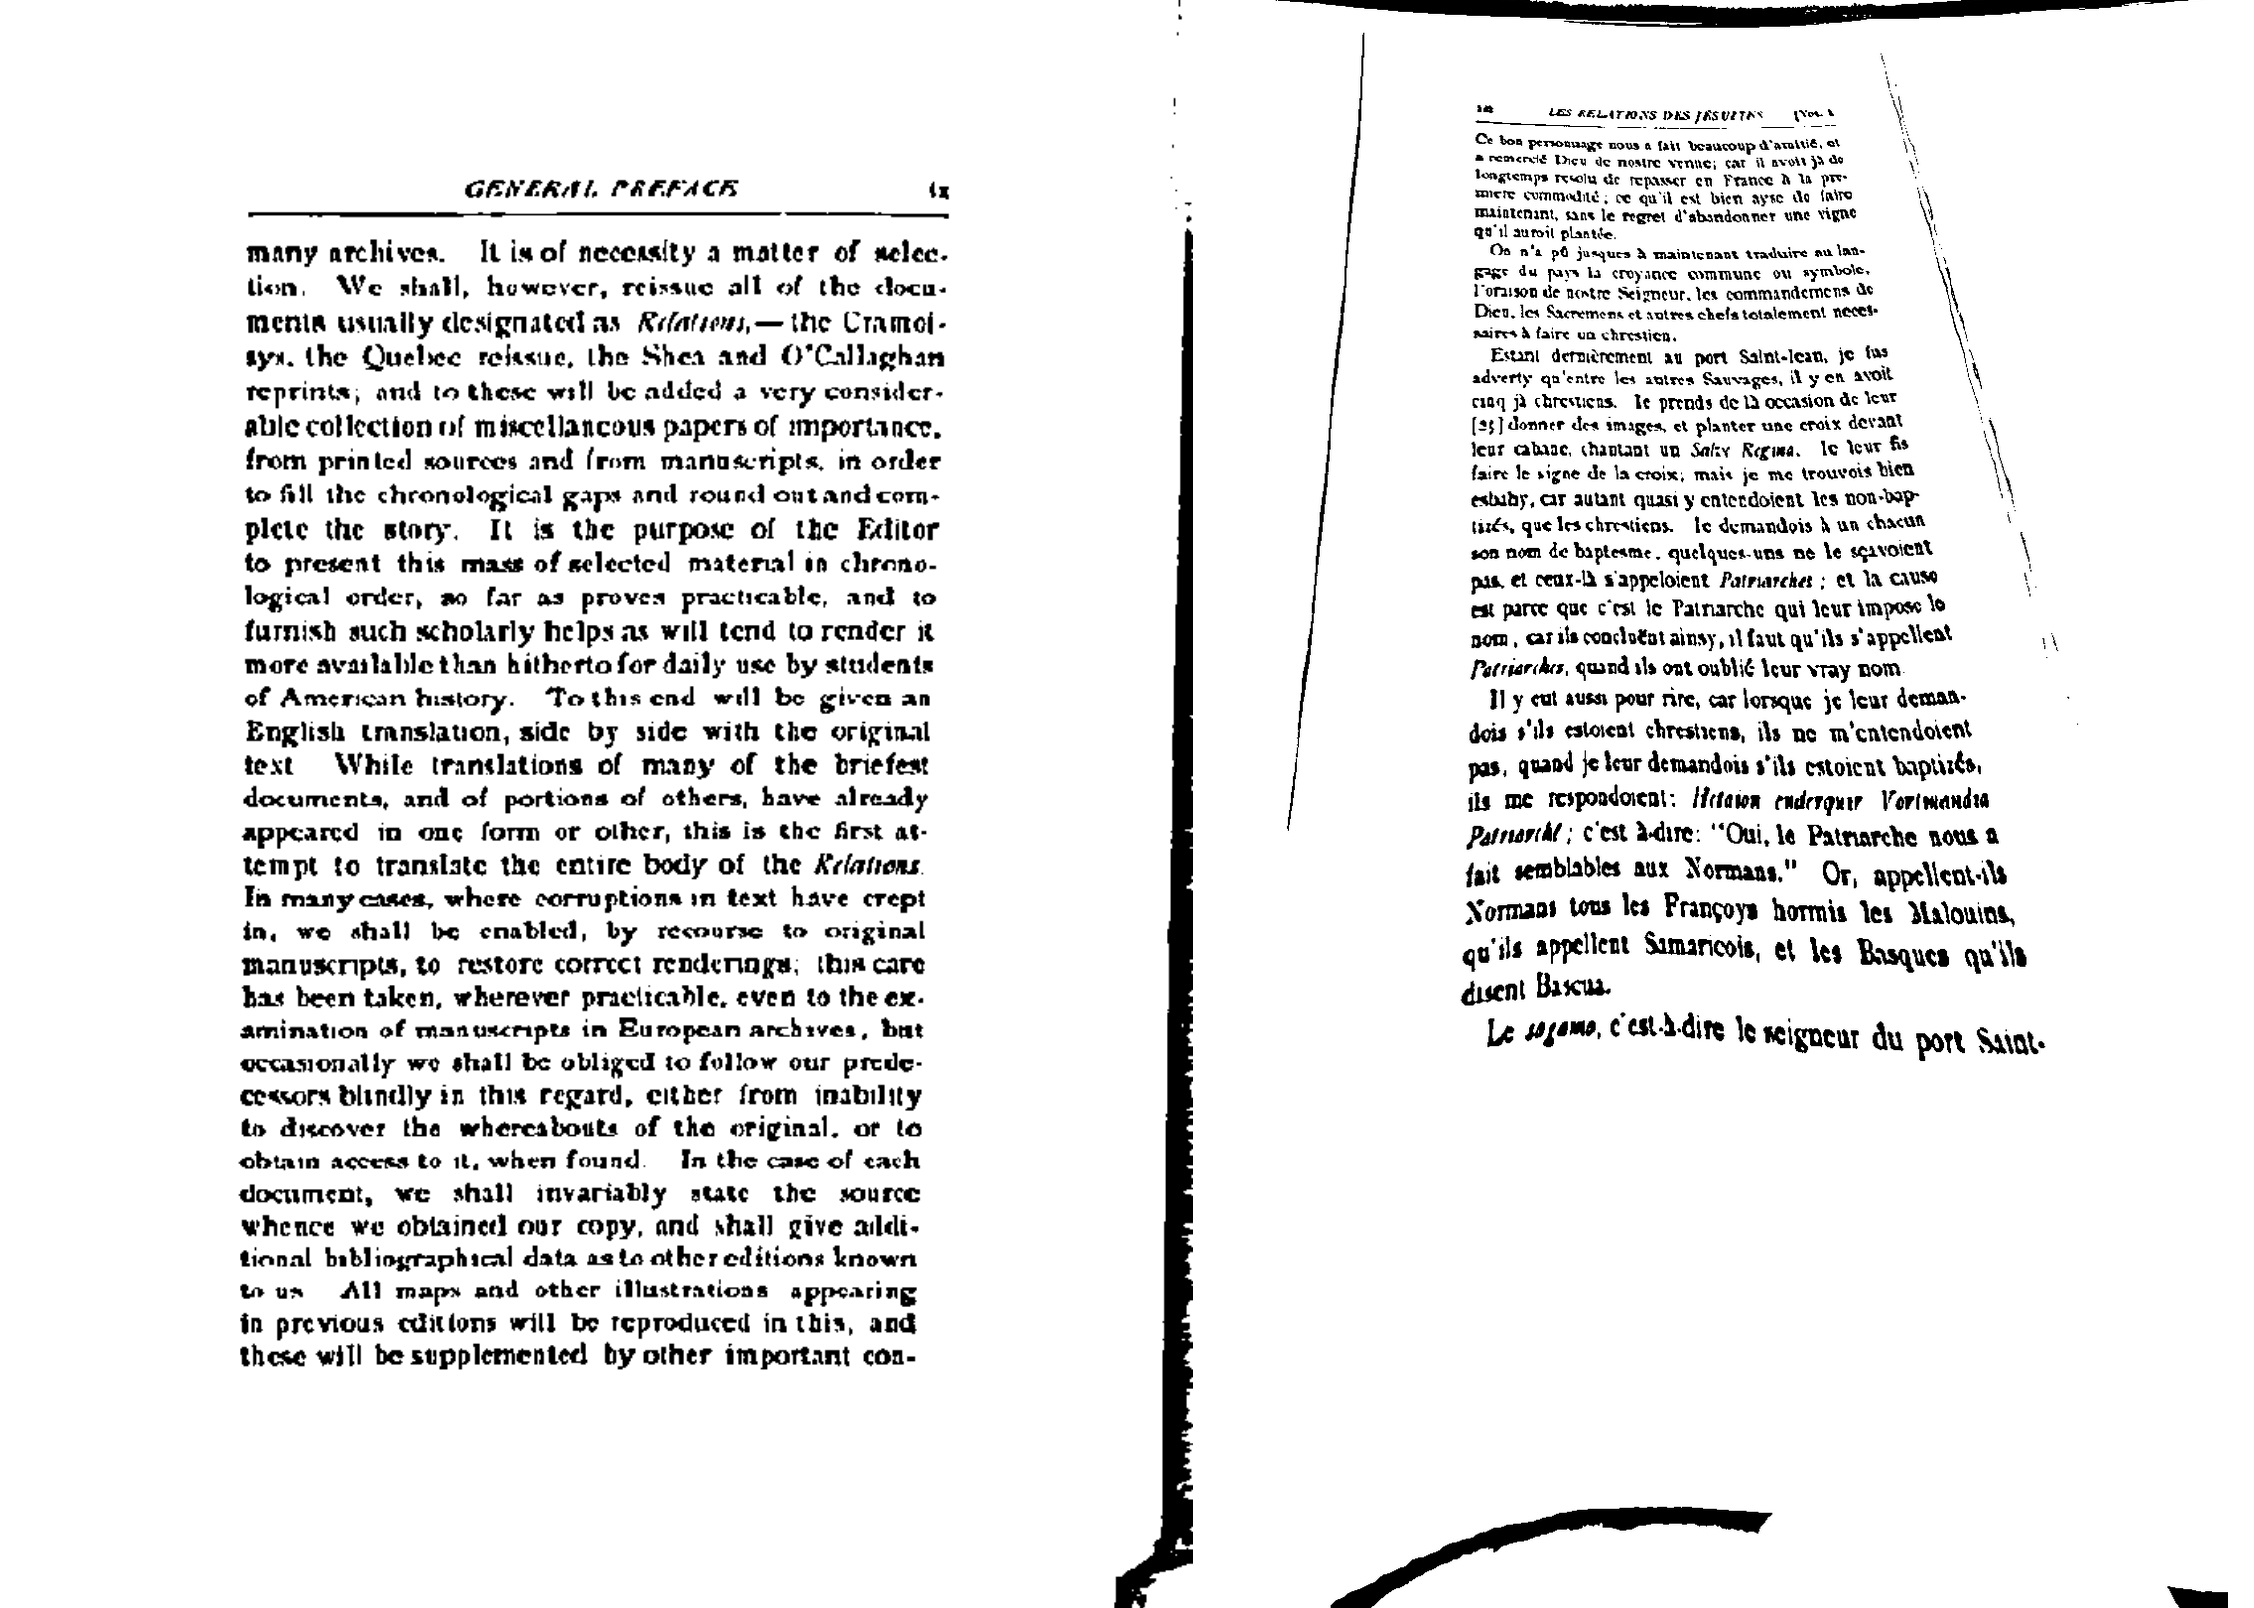
\includegraphics[width=1\linewidth]{scan.png}
    \caption{Examples of Successful and Unsucessful Scans: page14 (left) and page179 (right)}
    \label{fig:enter-label}
\end{figure}

I also conducted a simple file conversion, a series of jpeg files to a combined pdf file, utilizing img2pdf pip library. This effectively organizes the images into a single file. Nonetheless, I could merge it with the output of \texttt{page-dewarp}(after merging the series of png files to a combined pdf file utilizing img2pdf), prioritizing \texttt{page-dewarp} outputs, so that there would at least be the original images for the unscanned pages, serving as a fail-safe.\newline

Nonetheless, the proof of concept serves as a rudimentary model demonstrating how a video to pdf scanner may operate.\newline

\section{Metric and Evaluation}

Reliability of detecting PTEs is important and will be measured by comparing the known page number with the generated page number. Overall quality of the pdf will be examined by examining the pixel count of the scan. Book spine morphing, and margin consistency. These metrics will be measured automatically during development.\newline

It is imperative to measure the quality of the scan in an automated manner due to the large volume of data required to test at each iteration of machine learning.\newline

When testing \texttt{page-dewarp} python package, which is designed specifically to dewarp the spine curve of books from it's images. Often it would over-morph the image and generated document scans of inconsistent sometimes even diagonal left and right margins. Since the primary goal of the program is to morph the image into a flat document, evaluating the consistencies of the margins utilizing OCR would be ideal.\newline

This could be accomplished with an implementation of a pseudo-code such as this.\newline

\noindent{\texttt{leftMargins = [array of x-coordinates of the left most texts]}}\newline
\noindent{\texttt{rightMargins = [array of x-coordinates of the right most texts]}}\newline
   
\noindent{\texttt{standardDeviationLeft = statistics.stdev(leftMargins})\newline}
\noindent{\texttt{standardDeviationRight = statistics.stdev(rightMargins})\newline}

    
\noindent{\texttt{return {standardDeviationLeft, standardDeviationRight}}\newline}

The actual value of the margins need to be checked to ensure that the margin is not consistently near zero or near max-value, which may indicate that the text was cropped off. The vertical margins could also be evaluated in a similar manner to ensure that the program did not fail to morph the spine curve. And if so, to what extent it did.\newline

\section{Ethical Considerations}
\subsection{License}
All programs mentioned in the paper has either been under the Apache or the MIT License, which allows me to freely modify and use for any purposes.\newline

The git repository contains a rudimentary scans of the book, The Jesuit Relations and Allied Documents, that was published in 1896, and is under the public domain. In fact, a scan is available on \url{archive.org} \cite{archive2009}.\newline

\subsection{Misuse}
There is significant probability for misuse of the program as it could be used to scan and distribute copyrighted material, undermining intellectual property rights. Though the probability of the misuse is significant, the significance of misuse itself is dismal. The distribution copyrighted material on the internet is methodical and rampant. In other words, the quest of preserving non-commercial violations of intellectual property on the internet is a hopeless cause. And the project cannot conceivably have a significant impact on it.\newline

Though it could theoretically make privately sharing copies of texts such as a tediously specific edition of a textbook, yet to be pirated, among students and professors easier. I am specifically and deeply concerned by the misuse potential in the context of textbooks due to publishers' predatory practice of publishing new editions needlessly frequently, suffocating and disorienting the used textbook market. \newline

Nonetheless, to reiterate, I do no believe that the project will neither cause a significant influx the supply of stolen intellectual property nor have a significant impact on the print industry.  \newline

\subsection{Use of Copyrighted Material to Train the Model}
The training of the model may entail the use of copyrighted material, especially since the texts used in PUCIT dataset mostly consists of copyrighted books. Nonetheless, the project aims to create a product sufficiently transformative to be legally and morally defensible: the study aims to process footage of books to scan it, unlike Large Language Models which mimics and can at times even recreate the training dataset.\newline

\section{Weekly Schedule}
\rowcolors{3}{white}{gray!10}
\begin{tabular}{ |p{0.8cm}|p{5cm}| }
\hline
Week & Goal \\
\hline
\rowcolor{gray!10} 1 & code the margin pseudo-code\\
2 & test the reliability of the code by comparing it to manual analysis\\
3 & test Stony Brooks' DocUNet utilizing PUCIT\\
4 & create your own dataset akin to PUCIT)\\
5 & look into the code of \texttt{page-dewarp}\\
6 & create the fail-safe\\
7 & begin machine-learning\\
8 & Implement OCR (OpenCV + Tesseract)\\
9 & finalize the program\\
10 & run the program on various old books and collect data\\
11 & write the paper\\
12 & finalize the paper\\

\hline
\end{tabular}
  
\printbibliography
\end{document}
